\chapter{Experiments and Results}
\label{cha:ResearchAndResults}

This section will contain the results from the experiments. 

\section{Litterature search}
The litterature search yielded 123 studies of interest. Of these 25 had raw microRNA public. For the other studies, we sent an email requesting the raw miRNA data. However, only one such dataset were recieved, leading to an overall 26 datasets that are analyzed in this project (\py{", ".join(f"\\citep{{{study}}}" for study in studies)}).

The distribution of technologies in these different studies are visualized in \autoref{fig:technologies}. The number of samples are 

\begin{figure}
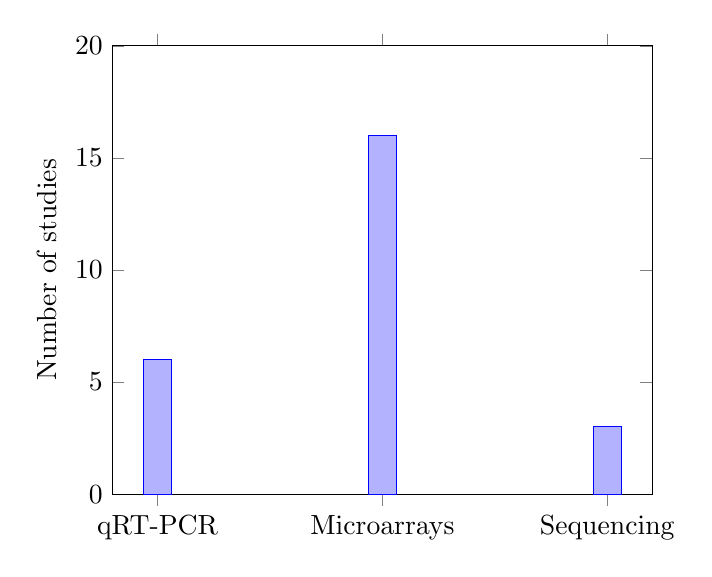
\begin{tikzpicture}
    \begin{axis}[
            ybar,
            symbolic x coords={qRT-PCR, Microarrays, Sequencing},
            xtick=data,
	    ylabel={Number of studies},
	    ymin=0,
	    ymax=20
        ]
        \addplot coordinates {(qRT-PCR, 6) (Microarrays, 16) (Sequencing, 3)};
    \end{axis}
\end{tikzpicture}
\label{fig:technologies}
\caption{Number of studies of each type}
\end{figure}

\begin{figure}
\begin{tikzpicture}
\begin{axis}[
    ybar stacked,
    legend style={at={(0.5,-0.20)},
      anchor=north,legend columns=-1},
    ylabel={Number of samples},
    reverse legend=true,
    legend style={cells={anchor=west}, legend pos=north east},
    table/col sep=comma,
    ymin=0,
    xtick=\empty,
%    ymode=log,
    width=\textwidth
    ]
    \addplot [fill=green] table [y=Controls, x expr=\coordindex] {tables/samples_count.csv};
    \addplot [fill=red] table [y=Cases, x expr=\coordindex] {tables/samples_count.csv};
\legend{Controls, Cases}
\end{axis}
\end{tikzpicture}
\end{figure}


\section{Processing the datasets}



\iffalse

\section{Experimental Plan}
\label{sec:experimentalPlan}

Trying and failing is a major part of research. However, to have a chance of success you need a plan driving the experimental research, just as you need a plan for your literature search. Further, plans are made to be revised and this revision ensures that any further decisions made are in line with the work already completed.  

The plan should include what experiments or series of experiments are planned and what question the individual or set of experiments aim to answer. Such questions should be connected to your research questions so that in the evaluation of your results you can discuss the results wrt to the research questions.  

\section{Experimental Setup}
\label{sec:experimentalSetup}

The experimental setup should include all data - parameters etc, that would allow a person to repeat your experiments. 

\section{Experimental Results}
\label{sec:experimentalResults}

Results should be clearly displayed and should provide a suitable representation of your results for the points you wish to make. Graphs should be labeled in a legible font and if more than one result is displayed on the same graph then these should be clearly marked.   Please choose carefully rather than presenting every results. Too much information is hard to read and often hides the key information you wish to present. Make use of statistical methods when presenting results, where possible to strengthen the results.  Further, the format of the presentation of results should be chosen based on what issues in the results you wish to highlight. You may wish to present a subset in the experimental section and provide additional results in the appendix.

\fi
